\chapter{Deep Generative Models}
Another type of unsupervised learning, in particular in the field of Deep Learning, are \textbf{Deep Generative Models (DGMs)}. The first important thing that we need to point, is the difference between the terms \textbf{generative} and \textbf{discriminative}. Generative models are statistical models of the data distribution \(p_X\) or \(p_{XY}\) depending on the availability of target data. Discriminative models are statistical models of the conditional distribution \(p_{X|Y}\) of the target given the input.

A discriminative model can be constructed from a generative model via the Bayes rule, but not vice versa!
\begin{equation}
    p_{Y|X}(y,x) = \frac {p_{XY} (x,y)} {\sum_{y'} p_{XY} (x,y')}
\end{equation}

\section{Density Estimation}
We are interested in the \textbf{Density Estimation}, in the case of the density estimation we are in the unsupervised learning setting, and we want to find the probability distribution \(f \in \Delta(\mathcal{Z})\) that fits the data \(z \in \mathcal{Z}\), where \(z\) is sampled from an unknown data distribution \(p_\text{data} \in \Delta(\mathcal{Z})\). Since in the unsupervised learning setting we don't have annotations, we have that \(\mathcal{Z} = \mathcal{X}\) (while in supervised learning \(\mathcal{Z} = \mathcal{X} \times \mathcal{Y}\).

The previous density estimation is called \textbf{explicit}, on the other hand, the \textbf{implicit} density estimation aims to find a function \(f \in \mathcal{Z}^\Omega\) that generates data \(f(\omega) \in \mathcal{Z}\) from an input \(\omega\) sampled from some predefined distribution \(p_\omega \in \Delta(\Omega)\) in a way that the distribution of generated samples fits the (unknown) data distribution \(p_\text{data} \in \Delta(\mathcal{Z})\).

\begin{figure}[h!]
    \centering
    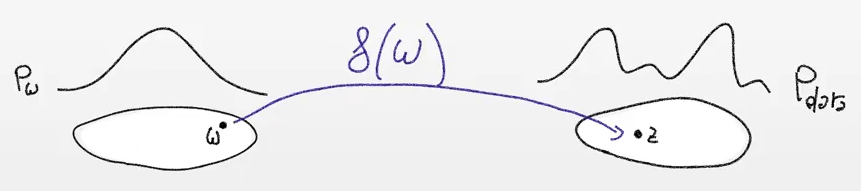
\includegraphics[width=.75\textwidth]{081}
    \caption{Implicit Desity Estimation.}
    \label{fig:081}
\end{figure}

The objective of the density estimation are: to define an hypothesis space \(\mathcal{H} \subset \Delta(\mathcal{Z})\) of models that can represent probability distributions (implicitly or explicitly); to define a divergence measure \(d \in \mathbb{R}^{\Delta(\mathcal{Z}) \times \Delta(\mathcal{Z})}\) between probability distributions in \(\Delta(\mathcal{Z})\) (e.g. Kullback-Leibler divergence); find an hypothesis \(q^* \in \mathcal{H}\) that best fits the data distributed according to \(p_\text{data}\). The best fit is measured using the divergence \(d\), i.e.:
\begin{equation}
    q^* \in \arg \min_{q \in \mathcal{H}} d(p_\text{data}, q)
\end{equation}
\begin{figure}[h!]
    \centering
    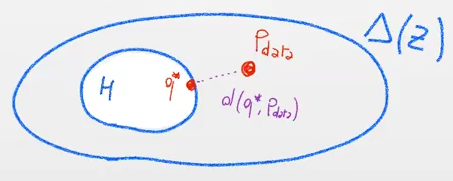
\includegraphics[width=.5\textwidth]{082}
    \caption{}
    \label{fig:082}
\end{figure}

Examples of algorithms that use density estimation are:
\begin{itemize}
    \item Variational AutoEncoder (VAE), that use explicit density, and
    \item Generative Adversarial Networks (GAN), that use implicit density.
\end{itemize}
These two algorithm both solve the same problems, but with different assumptions.

\section{Variational AutoEncoder (VAE)}
The idea of Variational AutoEncoder is to revisit autoencoder in a probabilistic fashion.

\subsection{AutoEncoder}
An autoencoder is a way of compressing high-dimensional data into a lower dimensional representation. An \textbf{encoder} maps input data \(x\) to a compressed representation \(\omega\). The compressed representation preserves meaningful factors of variations in the data. E.g. PCA with dimensions dropped can be seen as a linear encoder preserving as much variance in the data as possible. 

In this case we assume more complex transformations from the original space \(\mathcal{X}\) to the latent space \(\Omega\) that can be obtained with linear transformation and non-linearity.

An encoder is trained by leveraging a \textbf{decoder} mapping the representation \(\omega\) back to the input domain yielding \(\hat{x}\) (reconstruction). So, the decoder \emph{autoencodes} its input. the objective is to minimize the divergence between input \(x\) and its reconstruction \(\hat{x}\).

\begin{figure}[h!]
    \centering
    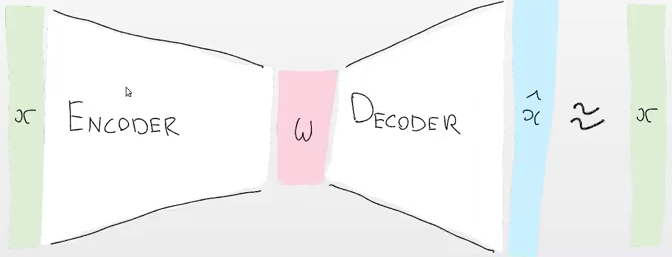
\includegraphics[width=.5\textwidth]{083}
    \caption{Encoding and Decoding functions representation.}
    \label{fig:083}
\end{figure}

After training the decoder is not needed anymore, since it was only functional to estimate the encoder. The encoder can be used to initialize or precompute features for supervised models.

\begin{figure}[h!]
    \centering
    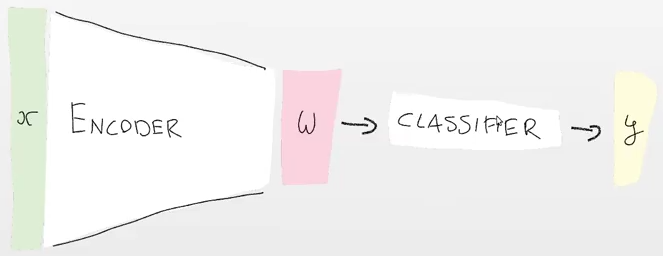
\includegraphics[width=.5\textwidth]{084}
    \caption{AutoEncoder usage.}
    \label{fig:084}
\end{figure}

\subsection{AutoEncoder in Generative Models}
AutoEncoders are generally used to train an encoder network that can be used for supervised learning purpose. But we are now interested on the usage of AutoEncoders for generate new data, infact the decoder could be used to generate new data, so AutoEncoders can be thought as a generative model, but it will not generate data according to the data distribution \(p_\text{data}\)!

What we would like to have is: given a latent space \(\Omega\) with a prior distribution \(p(\omega)\), and an input space \(\mathcal{X}\) with a data distribution \(p_\text{data}(x)\). We want a decoder that produce a mapping from the latent space to the input space where the regions of low probability of the latent input space correspond to the region of the low probability of the latent space, and the same thing with the region of high probability.

\begin{figure}[h!]
    \centering
    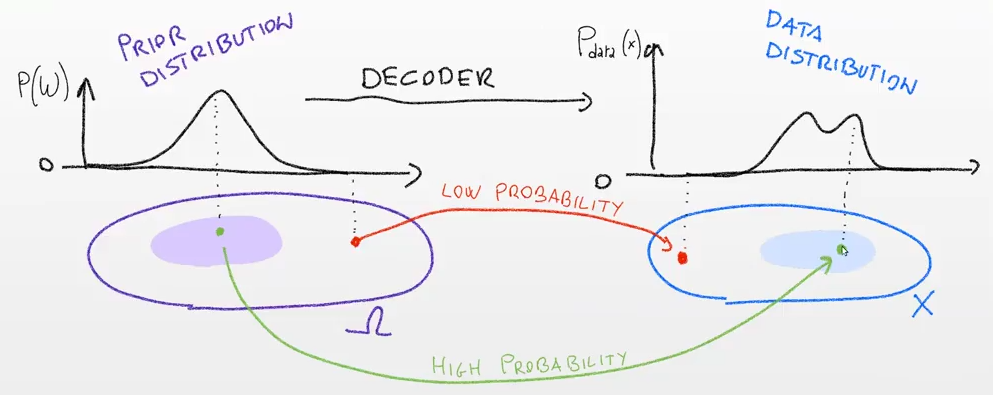
\includegraphics[width=.75\textwidth]{085}
    \caption{AutoEncoder usage.}
    \label{fig:085}
\end{figure}

Our problem can be formalized as follows: 
\begin{equation}
    q_\theta (x) = \mathbb{E}_{\omega \sim p_\omega} \left[ q_\theta (x | \theta) \right]
\end{equation}
Where \(\theta\) is our parameter, \(p_\theta\) is the priore, and \(q_\theta(x|\omega)\) is our decoder. Our objective is this optimization problem:
\begin{equation}
    \theta^* \in \arg \min_{\theta \in \Theta} d(q_\theta, p_\text{data})
\end{equation}
One possibility to measure the discrepancy (distance) of our prior data to our \(p_\text{data}\) is to use the Kullbakc-Leibler (KL) divergence:
\begin{equation}
    d_{KL}(p,q) = \mathbb{E}_{x \sim p} \left[ \log \frac {p(x)} {q(x)} \right]
\end{equation}

It turns out that this optimization is particularly difficult, in particular, we can make some calculations:
\begin{align}
    d_{KL} (p_\text{data}, q_\theta) &= \mathbb{E}_{x \sim p_\text{data}} \left[ \log \frac {p_\text{data}(x)} {q_\theta (x)} \right]\\
    &= - \mathbb{E}_{x \sim p_\text{data}} \left[ \log q_\theta(x) \right] + const\\
    &= - \mathbb{E}_{x \sim p_\text{data}} \left[ \log \mathbb{E}_{\omega \sim p_\omega} \left[ q_\theta(x | \omega) \right] \right] + const
\end{align}
but \( \mathbb{E}_{\omega \sim p_\omega} \left[ q_\theta (x | \omega) \right] \) is an intractable problem, therefore some trick are required.

We only need gradients for the optimization procedure, so, skipping all the derivations, we have that:
\begin{equation}
    \frac \delta {\delta \theta} d_{KL} (p_\text{data}, \_\theta) = - \mathbb{E}_{x \sim p_\text{data}} \mathbb{E}_{\omega \sim p_\omega} \left[ \frac {\frac \delta {\delta \theta} q_\theta (x | \omega)} { \mathbb{E}_{\omega \sim p_\omega} \left[ q_\theta (x | \omega) \right] } \right]
\end{equation}
now, we have problems with the expectation \( \mathbb{E}_{\omega \sim p_\omega} \left[ q_\theta (x | \omega) \right] \), that is still intractable, because we will have some sampling of \(\omega\) that will yield biased gradient estimates.

\subsection{Variational Upper Bound}
Let \(q_\psi (\omega | x) \in \Delta(\Omega)\), where \(\psi\) defines other parameters, denote an encoding probability distribution:
\begin{equation}
    \log \mathbb{E}_{\omega \sim p_\omega} \left[ q_\theta (x | \omega) \right] = \underbrace{ \mathbb{E}_{\omega \sim p_\psi(\cdot | x)} \left[ \log q_\theta (x | \omega) \right] }_\text{Reconstruction} - \underbrace{ d_{KL}(q_\psi(\cdot | x), p_\omega) }_\text{Regularizer}
\end{equation}
Now we can define a variational bound:
\begin{equation}
    d_{KL} (p_\text{data}, q_\theta) \leq \mathbb{E}_{x \sim p_\text{data}} \left[
        - \mathbb{E}_{\omega \sim p_\psi(\cdot | x)} [\log q_\theta (x | \omega)] + d_{KL}(q_\psi(\cdot | x), p_\omega)
    \right] + const
\end{equation}
The reconstruction is still intractable to compute, but is easy to get unbiased estimates of gradients with respect to \(\theta\) and \(\psi\). The regularizer might have closed-form solution, e.g. using gaussian distributions.

\begin{figure}[h!]
    \centering
    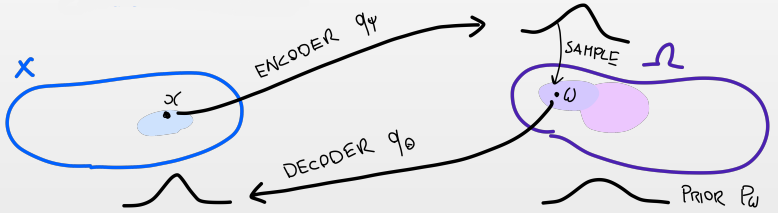
\includegraphics[width=.75\textwidth]{086}
    \caption{}
    \label{fig:086}
\end{figure}

\subsection{Conditional VAE}
Even if we are interested in unsupervised learning, Variational AutoEncoders can be extended also to cases in which we have side informations in our training set and we want to generate new data conditioned on these labels. Assume we have side information \(y \in \mathcal{Y}\) (e.g. digit labels) and we want to generate new data conditioned on the side information. We need to modify the encoder and decoder to take the side information in input obtaining \(q_\psi(\omega | x, y)\) and \(q_\theta(x | \omega, y)\). 

Similarly we can also define priors conditioned on side information \(p_\omega (\omega | y)\)

\begin{figure}[h!]
    \centering
    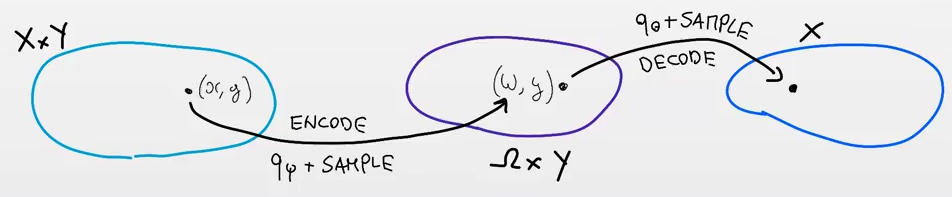
\includegraphics[width=.75\textwidth]{087}
    \caption{}
    \label{fig:087}
\end{figure}

\subsection{Issues with VAEs}
Despite VAEs are a very powerful technique to generate data and they are expecially good, they have some problems. For example, since they allow to move to the latent space, the generator tends to produce \textbf{blurry data}. Another problem is the problem of \textbf{underfitting}, in particular the balance between the regularization and the reconstruction terms must be managed carefully because if the regularizer is too strong, it will tend to be predominant and will tend to annihilate the model capacity.

\section{Generative Adversarial Networks (GAN)}
Generative Adversarial Networks are the most famous generative model, but they start from a different intuition from the Variational AutoEncoder, because the idea of having an implicit density model, so not requiring to estimate \(q_\theta(x)\).

GANs enable the possiblity of estimating implicit densities. We assome to have a prior density \(p_\omega \in \Delta(\Omega)\) and a generator (or decoder) \(g_\theta \in \mathcal{X}^\Omega\) that generates data points in \(\mathcal{X}\) given a random element from \(\Omega\).

The density induced by the prior \(p_\omega\) and the generator \(g_\theta\) is given by:
\begin{equation}
    q_\theta (x) = \mathbb{E}_{\omega \sim p_\omega} \delta \left[ g_\theta (\omega) - x \right]
\end{equation}
where \(\delta\) is the Dirac delta function.

\subsection{Objective}
The original GAN objective is to find \(\theta^*\) such that \(q_{\theta^*}\)best fits the data distribution \(p_\text{data}\) under the Jensen-Shannon divergence \(d_{JS}\), i.e.
\begin{equation}
    \theta^* \in \arg \min_\theta d_{JS} (p_\text{data}, q_\theta)
\end{equation}
where
\begin{equation}
    d_{JS} (p,q) = \frac 1 2 d_{KL} \left(
        p, \frac {p + q} 2
    \right) + \frac 1 2 d_{KL} \left(
        q, \frac {p + q} 2
    \right)
\end{equation}
Since our derivation is intractable to compute --- in particular we cannot compute the gradient of the distace, that allows us to train our generator --- we have to do some derivation that we will skip, but let's concentrate on the last formula:
\begin{align}
    d_{JS} (p,q) &= \frac 1 2 d_{KL} \left(
        p, \frac {p + q} 2
    \right) + \frac 1 2 d_{KL} \left(
        q, \frac {p + q} 2
    \right)\\
    &= \log (2) + \frac 1 2 \max_t \left\{
        \mathbb{E}_{x \sim p} \left[ \log t(x) \right] + \mathbb{E}_{x \sim q} \left[ \log (1 - t(x)) \right]
    \right\}
\end{align}
where \(t(x)\) is defined as \(t(x) = \frac {p(x)} {p(x) + q(x)}\), and is like a binary classifier predictin whether \(x\) came from \(p\) or \(q\). 

\subsubsection{GAN Objective Lower Bound}
Let \(t_\phi(x)\) be a classifier (or discriminator) for data point in \(\mathcal{X}\). Then we get the following lower boun on our objective:
\begin{align}
    d_{JS} (p,q) &= \log (2) + \frac 1 2 \max_t \left\{
        \mathbb{E}_{x \sim p_\text{data}} \left[ \log t(x) \right] + \mathbb{E}_{x \sim q_\theta} \left[ \log (1 - t(x)) \right]
    \right\}\\
    &\geq \log (2) + \frac 1 2 \max_\phi \left\{
        \mathbb{E}_{x \sim p_\text{data}} \left[ \log t_\phi(x) \right] + \mathbb{E}_{x \sim q_\theta} \left[ \log (1 - t_\phi(x)) \right]
    \right\}
\end{align}
Which is minimized to obtain the generator's parameter \(\theta^*\). Note that in this equation, the terms \(\log (2)\) and \(\frac 1 2\) can be neglected, because they are not changing the minimizer \(\theta^*\).
\begin{equation}
    \theta^* \in \arg \min_\theta \max_\phi \left\{
        \mathbb{E}_{x \sim p_\text{data}} \left[ \log t_\phi(x) \right] + \mathbb{E}_{x \sim q_\theta} \left[ \log (1 - t_\phi(x)) \right]
    \right\}
\end{equation}
Now note that we have the issue that this still depends on the explicit density \(q_\theta\), however we can equivalently rewrite it as
\begin{equation}
    \theta^* \in \arg \min_\theta \max_\phi \left\{
        \mathbb{E}_{x \sim p_\text{data}} \left[ \log t_\phi(x) \right] + \mathbb{E}_{\omega \sim q_\omega} \left[ \log (1 - t_\phi(g_\theta(\omega))) \right]
    \right\}
\end{equation}
Here we want to minimize the error of the discriminator in recognizing if a sample is real or fake, and we also want to push the generator \(g_\theta(\omega)\) to generate samples that are as close as possible to the real data.

\subsection{Issues with GANs}
The main problem with GAN is the \textbf{training stability}, because since we have the alternation between the generator and the discriminator, the parameters of the network may oscillate and never converge. 

Another problem is the \textbf{mode collapse}, the generator might learn to perfectly generate few examples from the training set, but not cover all the variability that is in the training set.

Finally, the last problem we will see, is the \textbf{vanishing gradient}, if the discriminator is very successful, then it will have a little gradient to learn, so it leaves the generator with little gradient to learn from, as we can see in Figure~\ref{fig:088}.

\begin{figure}[h!]
    \centering
    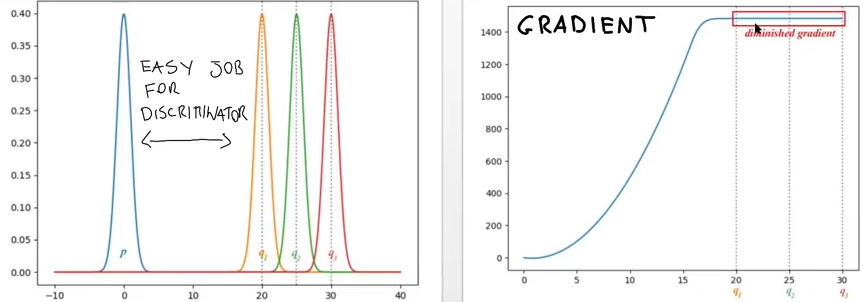
\includegraphics[width=.75\textwidth]{088}
    \caption{}
    \label{fig:088}
\end{figure}

\subsection{More GANs}
More GAN-like models can be constructed by considering different divergences between probabilities and by applying similar tricks to get rid of the necessity of knowing the explicit density:
\begin{itemize}[topsep={0pt}, partopsep={0pt}]
    \itemsep0pt
    \item \(f\)-GANs built on \(f\)-divergences.
    \item \(b\)-GANs built on Bergman divergences.
    \item Wasserstein GANs use the Wasserstein metric.
    \item Other GANs can be derived using integral probability metrics.
\end{itemize}
Furthermore, GANs and VAEs can be combined (VAE-GAN), and there exist conditional GANs that work like continual VAEs.

\newpage
\begin{exercise}
    \ex How can we use Autoencoders in generative models?
    \ex[!] Describe the Variational AutoEncoder and draw the model's framework.
    \ex What are the problems with VAE?
    \ex What part of the VAE do we use in test time?
    \ex[!] Describe the Generative Adversarial Networks and draw the model's framework.
    \ex What part of the GAN do we use in test time?
\end{exercise}